% ============================================================
%  TERM PROJECT — DEVELOPER DOCUMENTATION
%  Databases · THGA Bochum
% ============================================================
\documentclass[11pt,a4paper]{article}

\usepackage{thga-db}
\usepackage{graphicx}
\usepackage{float}

\renewcommand{\thgaKurs}{Databases}
\renewcommand{\thgaDatum}{Summer Term 2026}

\begin{document}
\thispagestyle{empty}

\thgaTitel{Term Project — Documentation}%
{VPN Access Manager}

\begin{infobox}
\textbf{Author:} Rayen Ben Haj Rhouma \\
\textbf{Module:} Introduction to Database Management Systems · THGA Bochum \\
\textbf{Stack:} PostgreSQL · FastAPI · Docker Compose · tkinter (\texttt{.deb}) \\
\textbf{Version:} 0.1.0 \\
\textbf{Repository:} \url{https://github.com/Rayen-CyberSecurity/vpn-access-manager}
\end{infobox}

\tableofcontents
\vspace{1em}

% ============================================================
\section{Introduction and motivation}
% ============================================================

VPN Access Manager is a small database application for managing VPN
connections across several gateways.

The system stores organisational departments, VPN users, gateways and VPN
sessions. It allows an administrator to see which sessions are currently
active, inspect previous sessions, open new sessions and close existing ones.

An important business rule is gateway capacity. Each gateway has a configured
maximum number of simultaneous active sessions. Before a new session is
created, the application verifies that the selected gateway still has
available capacity.

The project consists of three main components:

\begin{itemize}
    \item a \textbf{PostgreSQL} relational database,
    \item a \textbf{FastAPI} REST API,
    \item a \textbf{tkinter} desktop frontend.
\end{itemize}

The communication path is:

\begin{verbatim}
tkinter frontend  --->  FastAPI REST API  --->  PostgreSQL
                       HTTP / JSON
\end{verbatim}

The frontend never communicates directly with PostgreSQL. All database access
is performed by the API.

% ============================================================
\section{Data model}
% ============================================================

The relational model contains four entities.

\begin{description}

    \item[department]
    Represents an organisational department.

    \item[vpn\_user]
    Represents a person who may establish VPN sessions. The table is called
    \texttt{vpn\_user} rather than \texttt{user} to avoid confusion with the
    PostgreSQL user concept.

    \item[gateway]
    Represents a VPN gateway. Each gateway belongs to a region, has a public IP
    address and defines the maximum number of simultaneous sessions.

    \item[session]
    Represents one VPN connection between a user and a gateway.

\end{description}

A department can contain many VPN users.

A VPN user can have multiple sessions over time, and a gateway can also
participate in multiple sessions. The \texttt{session} table therefore
resolves the many-to-many relationship between users and gateways while also
storing attributes of the connection itself.

% ------------------------------------------------------------
\subsection{Relational schema}
% ------------------------------------------------------------

The implemented schema is:

\begin{verbatim}
department(
    id,
    name,
    contact_email
)

vpn_user(
    id,
    username,
    email,
    department_id -> department.id
)

gateway(
    id,
    name,
    region,
    public_ip,
    max_sessions
)

session(
    id,
    status,
    client_ip,
    connected_at,
    disconnected_at,
    bytes_transferred,
    user_id -> vpn_user.id,
    gateway_id -> gateway.id
)
\end{verbatim}

The primary keys are integer identifiers generated by PostgreSQL.

Foreign keys connect VPN users to departments and sessions to both users and
gateways.

\begin{figure}[H]
\centering
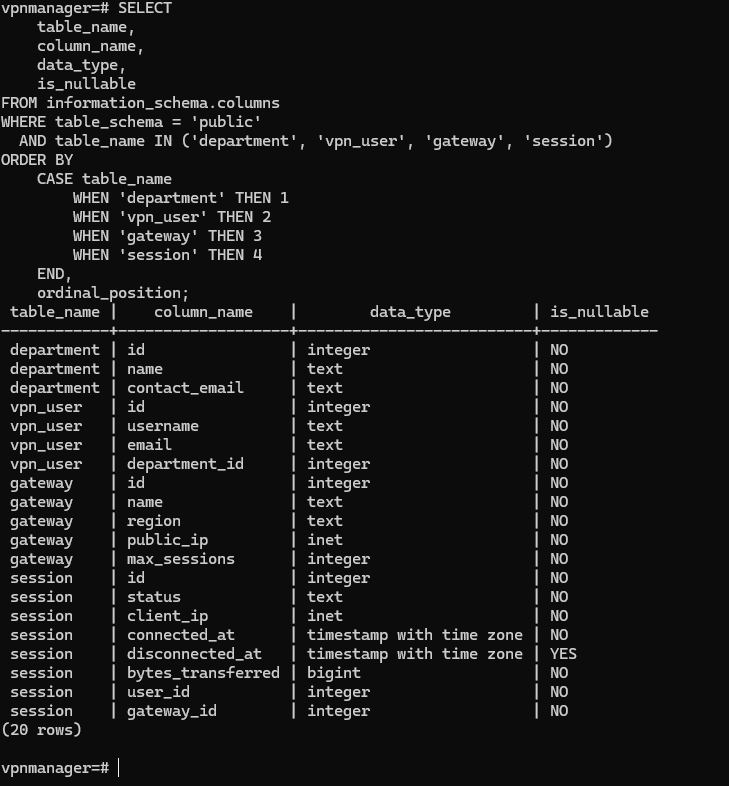
\includegraphics[width=\textwidth]{img/db-schema-check.png}
\caption{Implemented tables and columns in PostgreSQL.}
\end{figure}

% ============================================================
\section{Database implementation}
% ============================================================

The complete database definition and seed data are stored in
\texttt{db/init.sql}.

Docker Compose mounts this file into PostgreSQL's initialization directory.
When the database is created with a fresh volume, PostgreSQL executes the
script automatically.

This makes it possible to reproduce the initial database without manually
creating tables.

% ------------------------------------------------------------
\subsection{Database constraints}
% ------------------------------------------------------------

The schema uses primary keys, foreign keys, unique constraints and check
constraints to protect data integrity.

Important rules include:

\begin{itemize}

    \item \texttt{vpn\_user.username} is unique.

    \item \texttt{gateway.name} is unique.

    \item \texttt{gateway.max\_sessions} must be greater than zero.

    \item session status must be either \texttt{active} or \texttt{closed}.

    \item an active session cannot already have a disconnection timestamp.

    \item if \texttt{disconnected\_at} is present, it cannot be earlier than
          \texttt{connected\_at}.

    \item every session references an existing VPN user and gateway.

\end{itemize}

These rules prevent invalid records from being stored even if an incorrect
request reaches the database layer.

\begin{figure}[H]
\centering
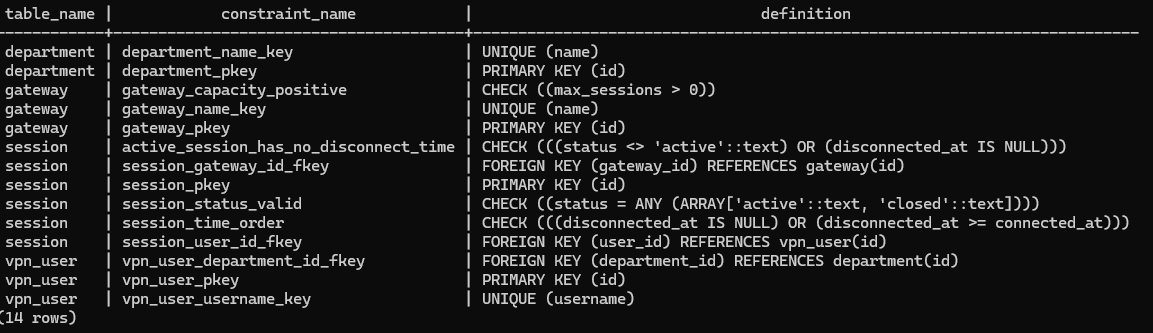
\includegraphics[width=\textwidth]{img/db-constraints.png}
\caption{Constraints defined on the four database tables.}
\end{figure}

% ------------------------------------------------------------
\subsection{Gateway capacity}
% ------------------------------------------------------------

Gateway capacity is different from the row-level constraints above.

The maximum number of active sessions depends on the number of
\emph{other session rows} that currently reference the same gateway.
Therefore, the rule is checked by the API before inserting a new session.

The API first retrieves the requested gateway and then counts its active
sessions.

Conceptually:

\begin{verbatim}
gateway = SELECT gateway by id

active = SELECT COUNT(*)
         FROM session
         WHERE gateway_id = requested gateway
           AND status = 'active'

if active >= gateway.max_sessions:
    reject request

otherwise:
    INSERT new active session
\end{verbatim}

If the gateway has reached its limit, the API returns HTTP status
\texttt{409 Conflict} and no session is inserted.

For example, if \texttt{gw-eu-1} has three active sessions and
\texttt{max\_sessions = 3}, another session request is refused.

% ============================================================
\section{REST API}
% ============================================================

The API is implemented with FastAPI.

Pydantic models are used for request validation and response models.
Database statements use parameters rather than inserting user-provided values
directly into SQL strings.

The project exposes exactly five REST operations:

\begin{center}
\begin{tabular}{|l|l|p{6cm}|}
\hline
\textbf{Method} & \textbf{Path} & \textbf{Purpose} \\
\hline
GET &
\texttt{/gateways} &
List gateways with their current active-session counts. \\
\hline

GET &
\texttt{/sessions} &
List sessions, optionally filtered by status or gateway. \\
\hline

GET &
\texttt{/sessions/\{id\}} &
Return one session and its related information. \\
\hline

POST &
\texttt{/sessions} &
Open a new VPN session. \\
\hline

POST &
\texttt{/sessions/\{id\}/close} &
Close an existing VPN session. \\
\hline
\end{tabular}
\end{center}

\begin{figure}[H]
\centering
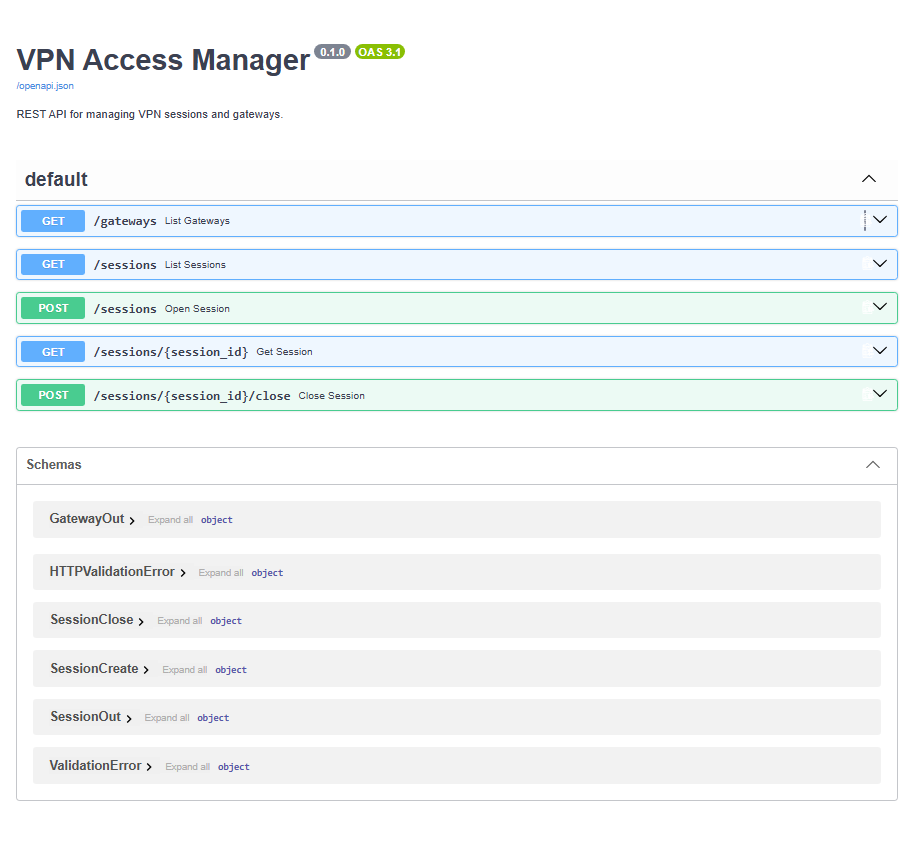
\includegraphics[width=\textwidth]{img/api-openapi-docs.png}
\caption{FastAPI OpenAPI documentation showing the five REST operations.}
\end{figure}

% ------------------------------------------------------------
\subsection{Reading sessions}
% ------------------------------------------------------------

The session list combines information from several tables.

The API joins:

\begin{verbatim}
session
vpn_user
department
gateway
\end{verbatim}

so that a client can receive useful information such as username, department
and gateway name without issuing separate requests.

The endpoint supports optional filters.

Examples:

\begin{verbatim}
GET /sessions?status=active
GET /sessions?gateway=gw-eu-1
GET /sessions?status=active&gateway=gw-eu-1
\end{verbatim}

% ------------------------------------------------------------
\subsection{Opening a session}
% ------------------------------------------------------------

A request to

\begin{verbatim}
POST /sessions
\end{verbatim}

contains:

\begin{verbatim}
{
    "user_id": 7,
    "gateway_id": 1,
    "client_ip": "192.168.50.10"
}
\end{verbatim}

Before insertion, the API verifies that the referenced user and gateway exist
and that the gateway has available capacity.

A successful creation returns HTTP status \texttt{201 Created}.

Invalid requests return an appropriate 4xx response.

% ------------------------------------------------------------
\subsection{Closing a session}
% ------------------------------------------------------------

A session is closed with:

\begin{verbatim}
POST /sessions/{id}/close
\end{verbatim}

Closing changes the status to \texttt{closed}, records the disconnection time
and stores the transferred byte count.

The operation is idempotent. If a session is already closed, another close
request returns the existing record without replacing its original closing
information.

% ------------------------------------------------------------
\subsection{API key}
% ------------------------------------------------------------

Read operations do not require authentication.

Operations that modify data require the HTTP header:

\begin{verbatim}
X-API-Key: <configured key>
\end{verbatim}

A missing or invalid key returns:

\begin{verbatim}
401 Unauthorized
\end{verbatim}

The expected key is loaded from the application configuration rather than
being written directly into an endpoint.

% ============================================================
\section{Database access and transactions}
% ============================================================

Database access is implemented with psycopg.

Two context managers are defined in \texttt{api/db.py}:

\begin{description}

    \item[query()]
    Opens a connection for read operations.

    \item[transaction()]
    Opens a connection for write operations and explicitly commits successful
    operations or rolls back when an exception occurs.

\end{description}

A simplified representation is:

\begin{verbatim}
with psycopg.connect(...) as conn:
    try:
        perform database operation
        conn.commit()
    except Exception:
        conn.rollback()
        raise
\end{verbatim}

This prevents a failed write operation from leaving a partially completed
change in the database.

% ============================================================
\section{Desktop frontend}
% ============================================================

The desktop frontend is implemented with tkinter.

It contains no SQL and does not import a PostgreSQL database driver. Instead,
\texttt{frontend/api\_client.py} provides a small HTTP wrapper around the
REST API.

The frontend consists of four principal screens:

\begin{enumerate}

    \item connection dialog,

    \item main gateway and session overview,

    \item new-session dialog,

    \item session-detail dialog.

\end{enumerate}

The main window displays gateway capacity and the session history.

\begin{figure}[H]
\centering
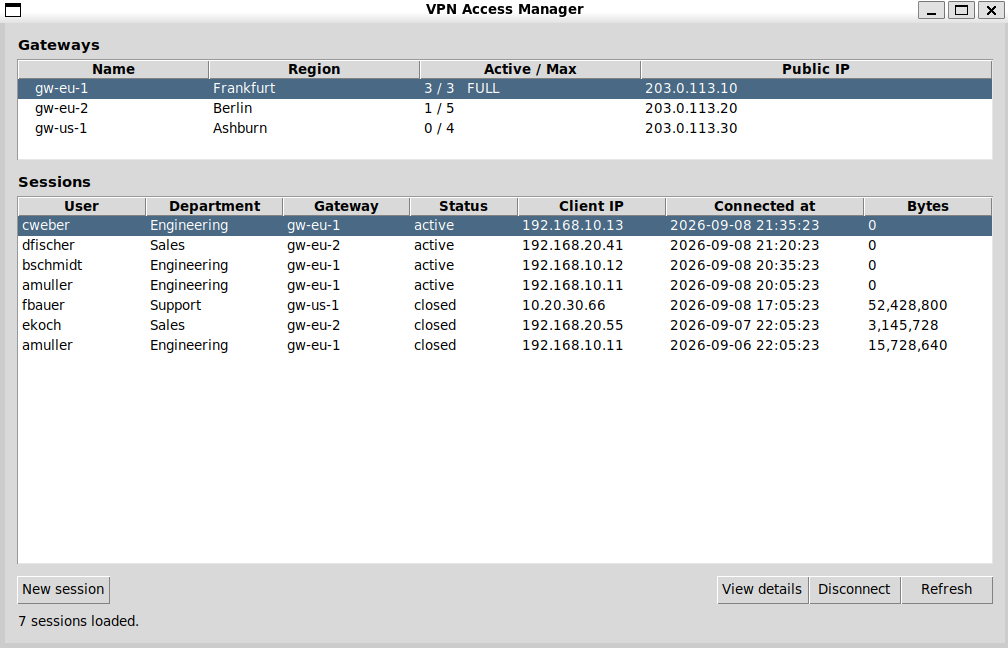
\includegraphics[width=\textwidth]{img/fe-main.png}
\caption{Desktop frontend showing gateway capacity and session information.}
\end{figure}

The available actions are:

\begin{itemize}
    \item open a new session,
    \item view session details,
    \item disconnect an active session,
    \item refresh the displayed data.
\end{itemize}

The frontend does not implement the capacity rule itself. The server remains
responsible for deciding whether a session may be created. If the API refuses
the request, the frontend displays the returned error message.

This keeps the business rule in one place instead of duplicating it in the
desktop application.

% ============================================================
\section{Docker deployment}
% ============================================================

Docker Compose is used to run PostgreSQL and the FastAPI service.

The application can be started with:

\begin{verbatim}
cp .env.example .env
docker compose up -d --build
\end{verbatim}

The PostgreSQL container uses a health check. The API service waits for the
database service to become healthy before starting.

The API is exposed on port:

\begin{verbatim}
8000
\end{verbatim}

FastAPI's interactive OpenAPI documentation is available at:

\begin{verbatim}
http://localhost:8000/docs
\end{verbatim}

Configuration values such as the database connection URL and API key are
loaded from environment variables.

% ============================================================
\section{Testing}
% ============================================================

The automated test suite uses pytest and FastAPI's TestClient.

The tests cover the principal acceptance criteria of the project, including:

\begin{itemize}

    \item the five required API operations,

    \item gateway active-session counts,

    \item gateways with zero active sessions,

    \item session retrieval,

    \item status filtering,

    \item gateway filtering,

    \item opening a valid session,

    \item rejection of nonexistent users or gateways,

    \item rejection when a gateway is at capacity,

    \item API-key protection for write operations,

    \item closing a session,

    \item idempotent repeated closing,

    \item database constraints.

\end{itemize}

The final test run contains 30 passing tests.

\begin{figure}[H]
\centering
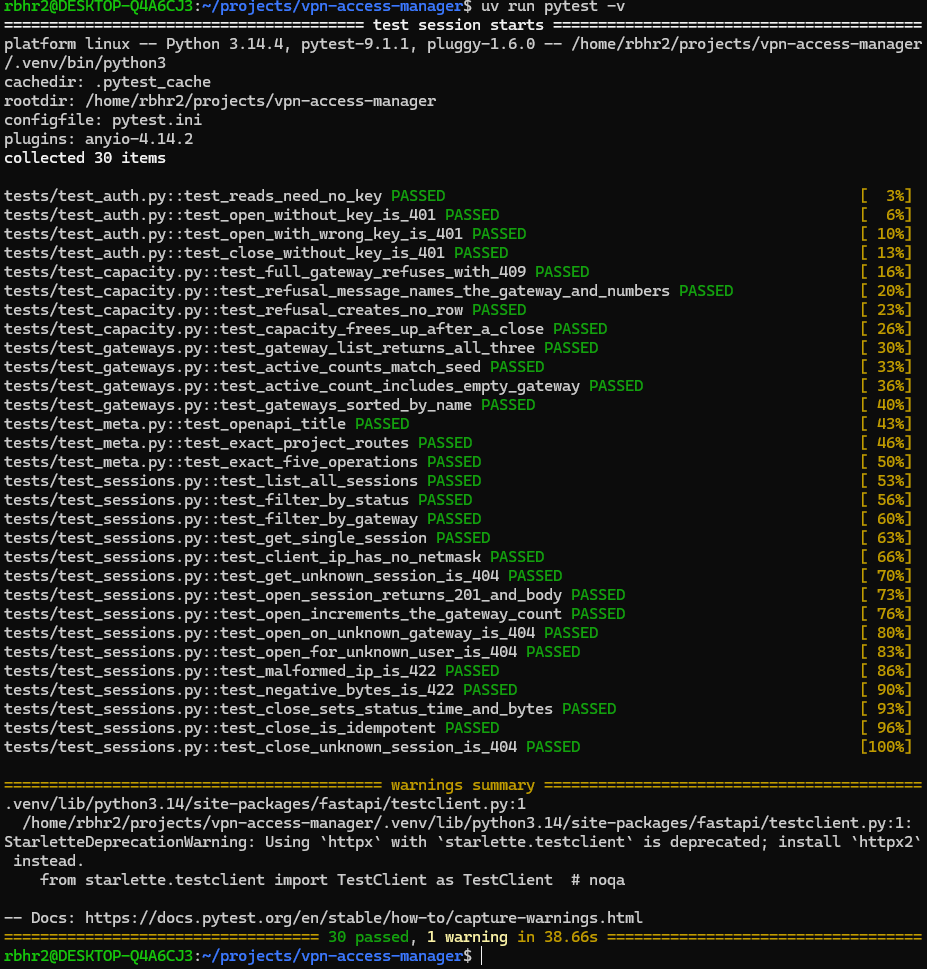
\includegraphics[width=\textwidth]{img/test-suite-green.png}
\caption{Final pytest run: all 30 tests pass.}
\end{figure}

The test database is reset from \texttt{db/init.sql}, providing a predictable
seed state for the tests.

% ============================================================
\section{Desktop packaging}
% ============================================================

The tkinter client is distributed as a Debian package.

The packaging script is:

\begin{verbatim}
frontend/packaging/build-deb.sh
\end{verbatim}

PyInstaller first creates the executable application. The script then stages
the executable together with its desktop entry and uses \texttt{fpm} to
produce:

\begin{verbatim}
vpn-manager_0.1.0_amd64.deb
\end{verbatim}

The package declares the required Linux graphical libraries as Debian
dependencies.

After installation, the client can be started with:

\begin{verbatim}
vpn-manager
\end{verbatim}

% ============================================================
\section{Project structure}
% ============================================================

The main project files are organised as follows:

\begin{verbatim}
vpn-access-manager/
|
|-- api/
|   |-- config.py
|   |-- db.py
|   |-- main.py
|   |-- models.py
|   `-- security.py
|
|-- db/
|   `-- init.sql
|
|-- frontend/
|   |-- api_client.py
|   |-- app.py
|   `-- packaging/
|       `-- build-deb.sh
|
|-- tests/
|
|-- docs/
|   |-- developer-doc.tex
|   |-- user-manual.tex
|   `-- img/
|
|-- docker-compose.yml
|-- Dockerfile
|-- requirements.txt
|-- pyproject.toml
`-- Makefile
\end{verbatim}

This separation keeps database definition, API logic, user interface,
automated tests and documentation independent from each other.

% ============================================================
\section{Reflection and limitations}
% ============================================================

The project demonstrates how database constraints and application-level
business rules complement each other.

Rules concerning a single stored value or row are enforced directly by
PostgreSQL where possible. Gateway capacity, however, requires counting active
session rows and is therefore checked by the API before a new session is
inserted.

Transactions are used for write operations so that unsuccessful operations
can be rolled back.

The REST API also creates a clear boundary between the database and the user
interface. The desktop application does not need to know the database schema
or PostgreSQL credentials.

The project deliberately remains small. It records VPN session information,
but it does not establish real VPN tunnels, authenticate against a real VPN
server, or collect network traffic automatically.

A single API key protects write operations. Per-user authentication and roles
are outside the scope of this version.

Possible future extensions include:

\begin{itemize}
    \item individual administrator accounts and roles,
    \item integration with real VPN gateways,
    \item automatic collection of traffic statistics,
    \item reporting and utilisation dashboards.
\end{itemize}

% ============================================================
\section*{Sources and reuse}
% ============================================================

The implementation uses the documentation of PostgreSQL, FastAPI, Pydantic,
psycopg, Docker, PyInstaller and fpm as technical references.

The document style and Makefile structure were adapted from the DBMS course
material.

All application-specific database design, API implementation, frontend,
tests and project documentation were produced for this term project.

\end{document}
